% !TeX spellcheck = da_DK
Dette kapitel vil beskrive systemets arkitektur.
Systemet er delt i to dele, én på computeren og en på NXT'en.


\begin{figure}[H]
\centering
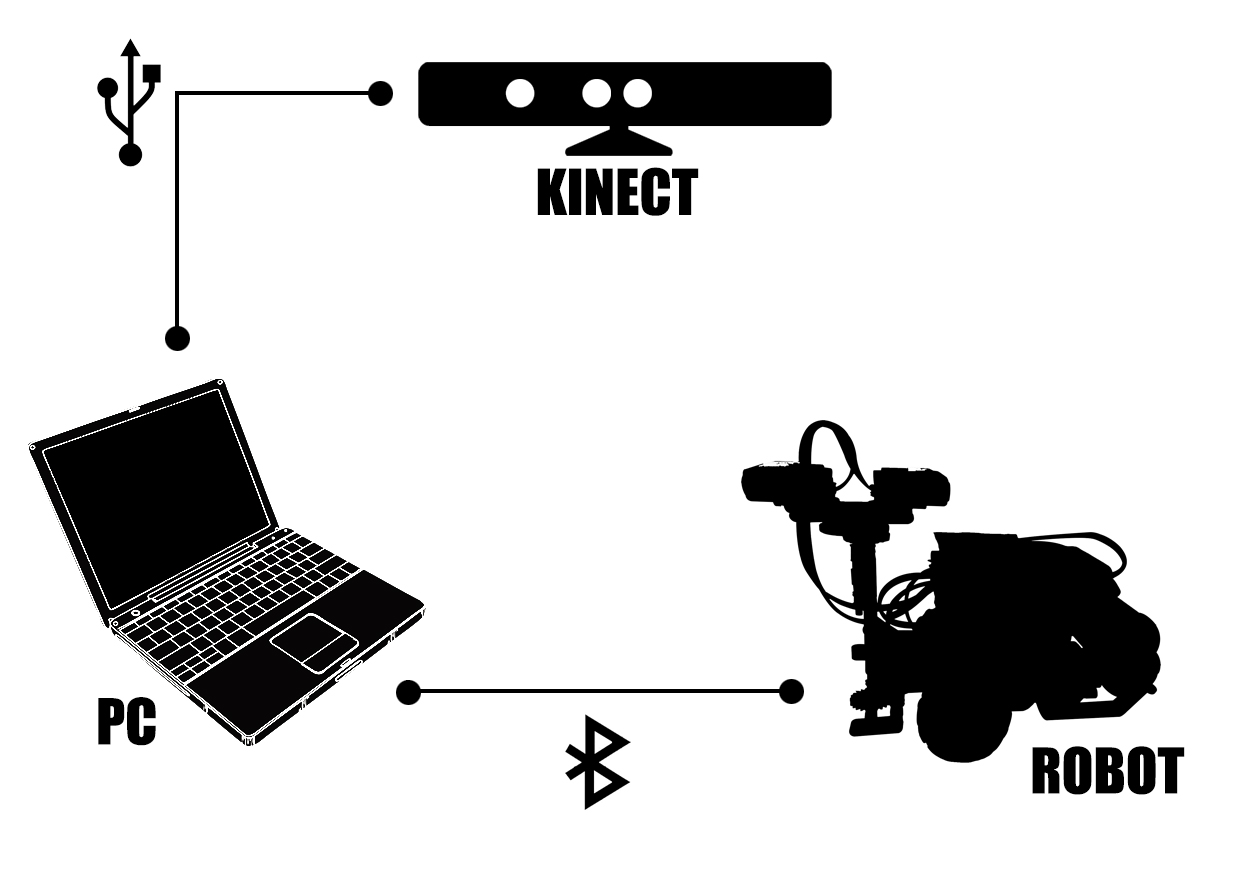
\includegraphics[width=1.0\textwidth]{enheder}
\caption{Systemets opbygning.}
\label{arkitektur:opbygning}
\end{figure}

Den overordnede opbygning af systemet kan ses på \cref{arkitektur:opbygning}.
Selve kortlægningen sker på computeren hvor occupancy grid algoritmen køres.
Computeren får sine oplysninger fra robotten gennem en bluetooth forbindelse.
Computeren bruger det grid, der er konstrueret til at fortælle robotten hvor den skal køre hen.
Computeren hjælper robotten med at fortælle den hvor den er, ved at fortolke et billede fra Kinecten og sende denne oplysning til robotten, hver gang den beder om det.
Når robotten er kommet frem til et punkt foretager den en sensormåling og sender denne tilbage til computeren.

I de følgende afsnit vil arkitekturen på henholdsvis NXTen og computeren blive beskrevet.

